\documentclass[fleqn,10pt]{SelfArx} % Document font size and equations flushed left

\usepackage{float}
\usepackage{graphicx}
\usepackage{caption}
\graphicspath{{../figures/}}


\definecolor{color1}{RGB}{0,0,90} % Color of the article title and sections
\definecolor{color2}{RGB}{0,20,20} % Color of the boxes behind the abstract and headings

\JournalInfo{Supplementary Text} % Journal information ``Journal, Vol. XXI, No. 1, 1-5, 2015''
\Archive{ } % Additional notes (e.g. copyright, DOI, review/research article)

\PaperTitle{Supplementary results for: A meta-analysis of computational biology benchmarks reveals publication bias affects on speed and accuracy} % Article title

\Authors{Paul P. Gardner\textsuperscript{1,2}*, James Paterson\textsuperscript{1,2}, Fatemeh Ashari Ghomi\textsuperscript{1,2}, Sinan Uğur Umu\textsuperscript{1,2}, Stephanie McGimpsey\textsuperscript{1,2}} % Authors
\affiliation{\textsuperscript{1}\textit{School of Biological Sciences, University of Canterbury, Christchurch, New Zealand.}} % Author affiliation
\affiliation{\textsuperscript{2}\textit{Biomolecular Interaction Centre and the Bio-Protection Research Centre, University of Canterbury, Christchurch, New Zealand.}}
\affiliation{*\textbf{Corresponding author}: paul.gardner@canterbury.ac.nz} % Corresponding author

\Keywords{computational biology --- accuracy --- benchmarks --- meta-analysis --- software development} % Keywords - if you don't want any simply remove all the text between the curly brackets
\newcommand{\keywordname}{Keywords} % Defines the keywords heading name

%----------------------------------------------------------------------------------------
%	ABSTRACT
%----------------------------------------------------------------------------------------

\Abstract{.}

\begin{document}

\flushbottom % Makes all text pages the same height
\maketitle % Print the title and abstract box
%\tableofcontents % Print the contents section

\thispagestyle{empty} % Removes page numbering from the first page

%----------------------------------------------------------------------------------------
%	ARTICLE CONTENTS
%----------------------------------------------------------------------------------------

\section*{Introduction} % The \section*{} command stops section numbering


XXXX





\clearpage
\newpage

\onecolumn

\section*{R code for Figure~1A\&B}

{\tiny
\begin{verbatim}

#read data
d <-read.table("meanRankSpeedData.tsv", header=T)

#initialize matrices
dNames <- c("IF", "H5", "relAge",       "yearPublished", "cites", "relCites",       "mindex",  "hindex",  "accuracyRank",  "speedRank" )
pNames <- c("JIF", "JH5", "Rel. age", "Year",          "Cites", "Rel. cites", "M-index", "H-index", "Accuracy",      "Speed")
pvalMatrix<-matrix(1, length(dNames), length(dNames))
rhoMatrix <-matrix(0, length(dNames), length(dNames))
sigMatrix <-matrix("",length(dNames), length(dNames))

colnames(pvalMatrix)<-pNames
rownames(pvalMatrix)<-pNames
colnames(rhoMatrix) <-pNames
rownames(rhoMatrix) <-pNames
colnames(sigMatrix) <-pNames
rownames(sigMatrix) <-pNames

#loop through pairwise combinations, record rho and P-values 
for(i in 1:length(dNames)){
      for(j in 1:length(dNames)){
	    spear<-cor.test(d[,dNames[i] == colnames(d)], d[,dNames[j] == colnames(d)], method = "spearman", exact = T)   #, alternative = "less")
	    pvalMatrix[i,j] <- spear$p.value 
	    rhoMatrix[i,j]  <- spear$estimate
	    if(spear$p.value < 0.05){
		sigMatrix[i,j]  <- "X"
	    }
      }
}

#generate plots
pdf(file=    "../figures/spearmanHeatmap.pdf", width = 7,  height = 6)
par(mar = c(8,4,4,4) + .1) #c(bottom, left, top, right). default: c(5, 4, 4, 2) + 0.1
heatmap.2(rhoMatrix, cellnote=sigMatrix,notecex=1.5,notecol="black", col=redblue(40), density.info="none", trace="none", dendrogram=c("column"), symm=F,symkey=T,symbreaks=T,
	scale="none", key.title = "", srtRow=45, adjRow=c(0, 1), srtCol=45, adjCol=c(1,1), breaks=(-20:20)/20,
margins = c(8, 8), cexRow=1.5, cexCol=1.5)
dev.off()

relCitesA<-cor.test(1-d$accuracyRank, as.numeric(d$relCites),     method = "spearman")
hindexA  <-cor.test(1-d$accuracyRank, as.numeric(d$hindex),       method = "spearman")
mindexA  <-cor.test(1-d$accuracyRank, as.numeric(d$mindex),       method = "spearman")
H5A      <-cor.test(1-d$accuracyRank, as.numeric(d$H5),           method = "spearman")
relAgeA  <-cor.test(1-d$accuracyRank, as.numeric(d$relAge),       method = "spearman")
speedA   <-cor.test(1-d$accuracyRank, as.numeric(d$speedRank),    method = "spearman")
citesA   <-cor.test(1-d$accuracyRank, as.numeric(d$cites),        method = "spearman")
IFA      <-cor.test(1-d$accuracyRank, as.numeric(d$IF),           method = "spearman")
yearA    <-cor.test(1-d$accuracyRank, as.numeric(d$yearPublished),method = "spearman")

pdf(file=    "../figures/spearmanBarplot.pdf", width = 5,  height = 3)
op<-par(mfrow=c(1,1),cex=1.0,las=2)
barplot(t(c(mindexA$estimate, hindexA$estimate, relAgeA$estimate, H5A$estimate, speedA$estimate, citesA$estimate, relCitesA$estimate, yearA$estimate, IFA$estimate)),
	names=c("M-index", "H-index", "Rel. age", 'JH5', "Speed", "Cites", "Rel. cites", "Year", "JIF"), ylab="Spearman's rho",ylim=c(-0.1,0.1),main="Correlates with accuracy rank")
lines(c(-100,100),c(0,0))
dev.off()
\end{verbatim}
}


\clearpage
\newpage

\begin{figure}[H]
\centering
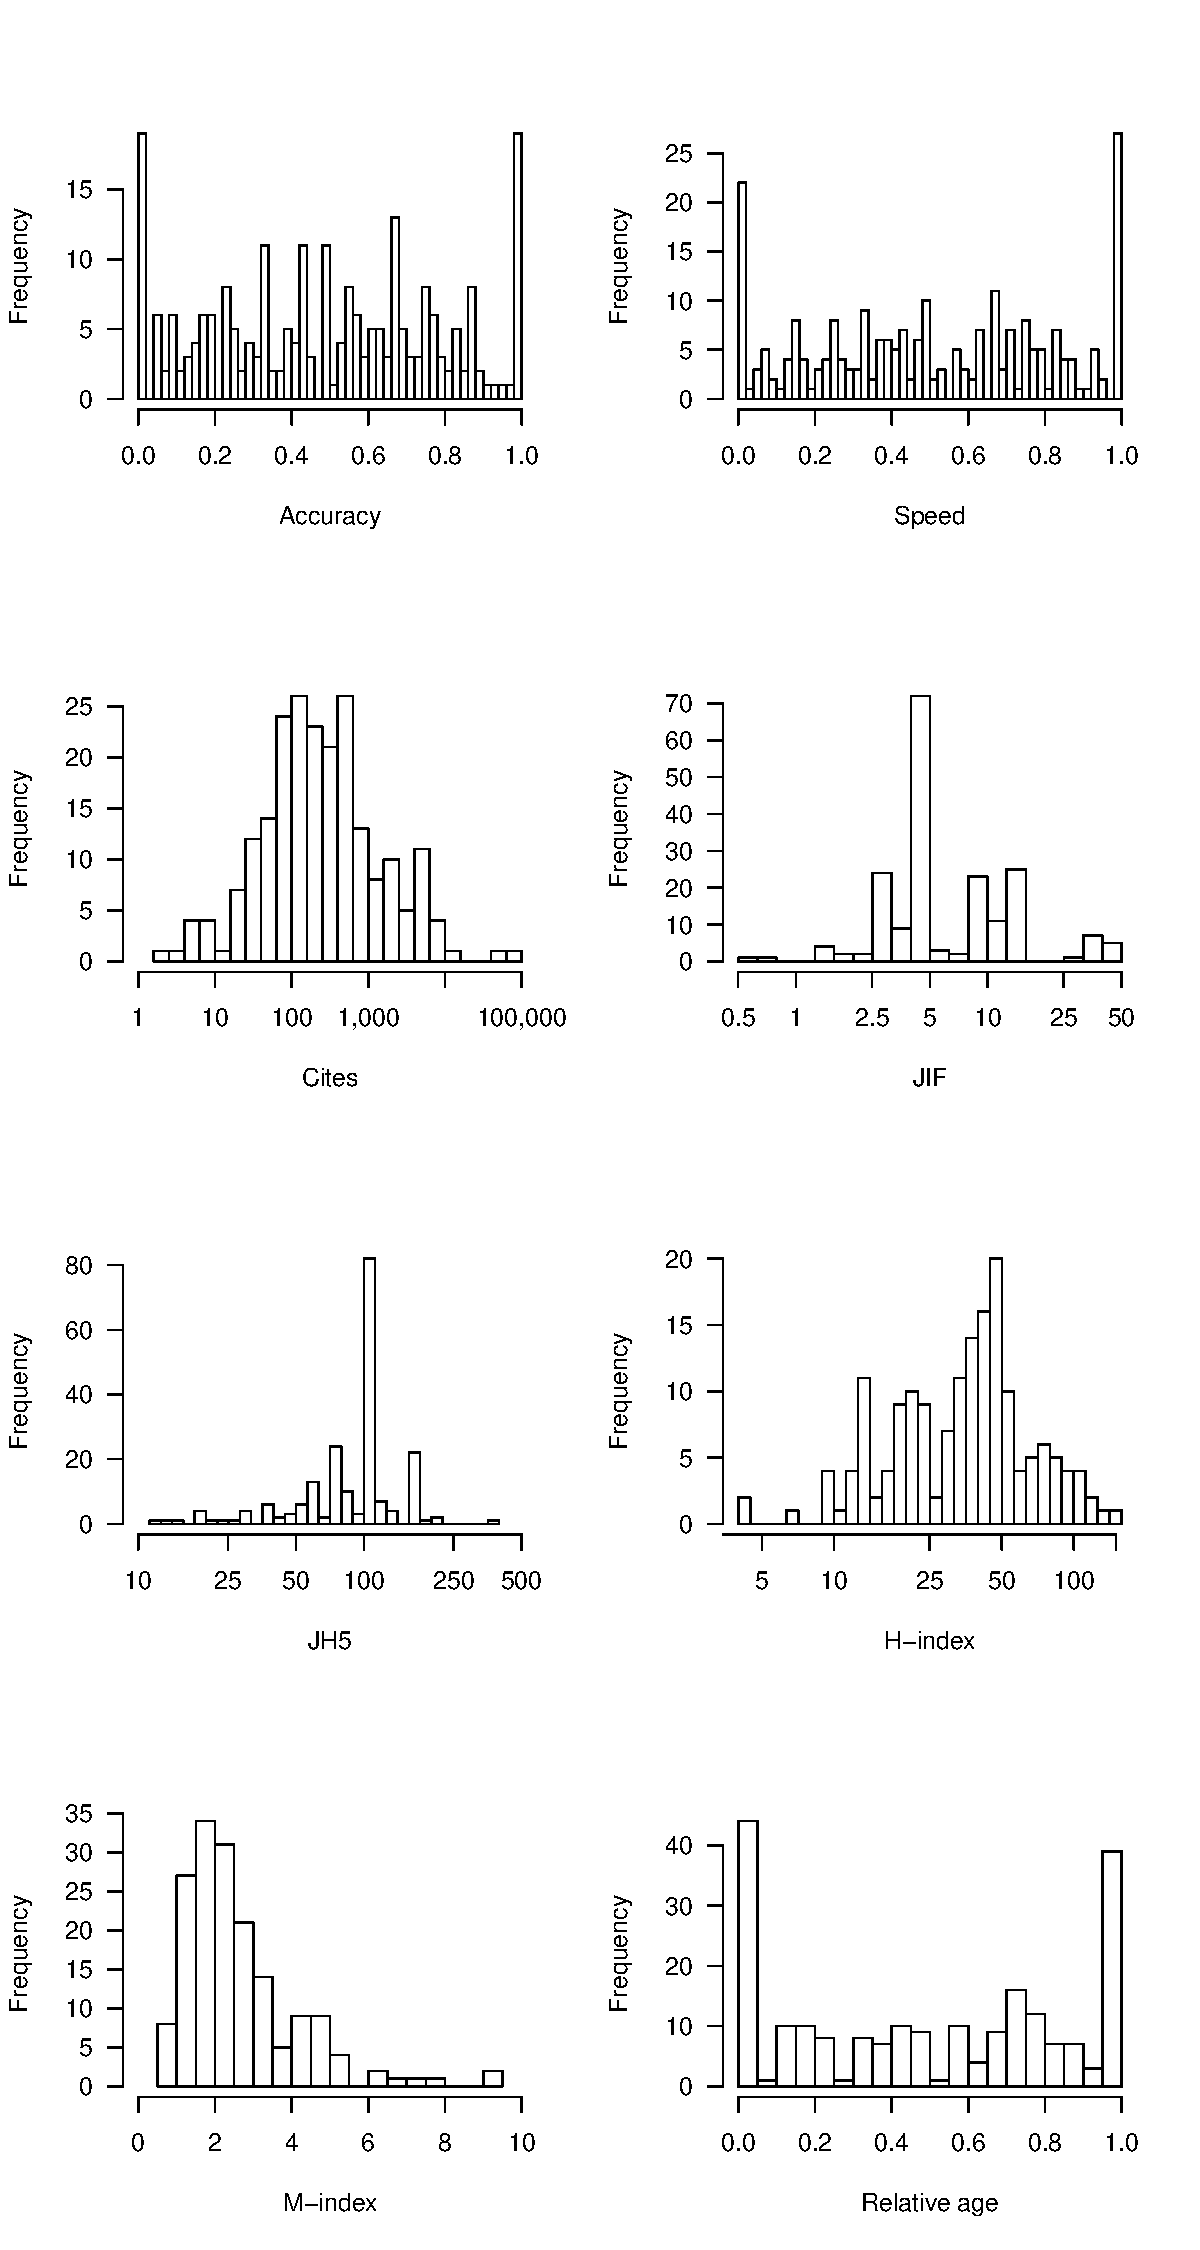
\includegraphics[width=0.55\textwidth]{supplementary-figures-small.pdf}
\caption{The distributions for the metrics used in this study. These
are, reading from left to right, top to bottom: Accuracy -- the mean
normalised accuracy rank for each benchmarked method; Speed -- the
mean normalised speed rank for each benchmarked method; Cites -- the number of
citations to the most cited manuscript describing a method, data from GoogleScholar;
JIF -- the Journal Impact Factor to the highest impact journal that has published
a manuscript describing a method, data from 2014 Thompson-Reuters Citation Reports;
JH5 -- the Journal H5 index to the highest impact journal that has published
a manuscript describing a method, data from GoogleScholar 2015 Metrics;
H-index -- the H-index for the highest profile corresponding author from the
manuscripts describing a method, data from GoogleScholar User Profiles;
M-index -- the M-index (H-index/(\#years since first publication)) for the
highest profile corresponding author from the manuscripts describing a method,
data from GoogleScholar User Profiles;}
\label{fig:S1}
\end{figure}



\begin{figure}[H]
\centering
\includegraphics[width=0.5\textwidth]{smoothScatter-speed-vs-accuracy.pdf}
\caption{...}
\label{fig:S2}
\end{figure}

\begin{figure}[H]
\centering
\includegraphics[width=0.85\textwidth]{smoothScatters.pdf}
\caption{...}
\label{fig:S3}
\end{figure}



\begin{figure}[H]
\centering
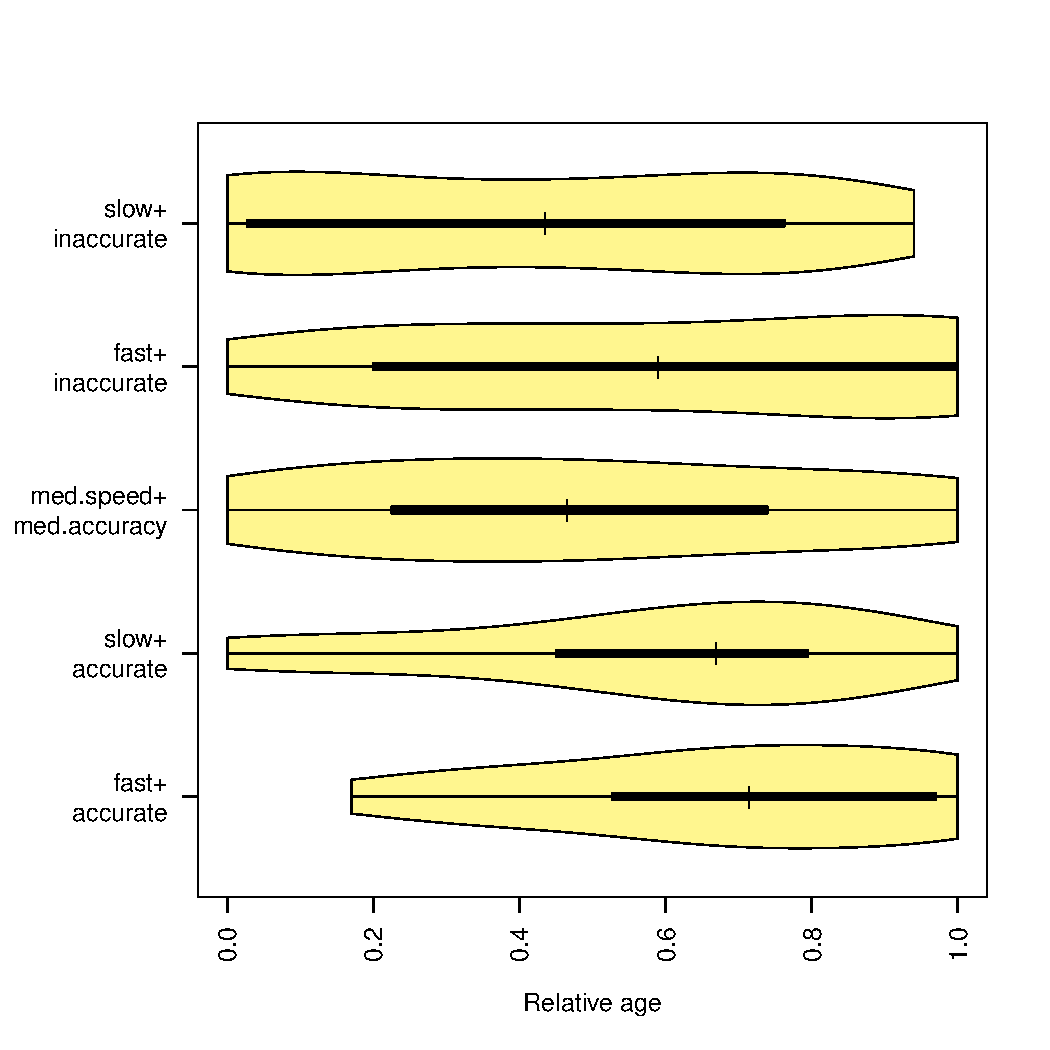
\includegraphics[width=0.45\textwidth]{relAge-speedAcc.pdf}
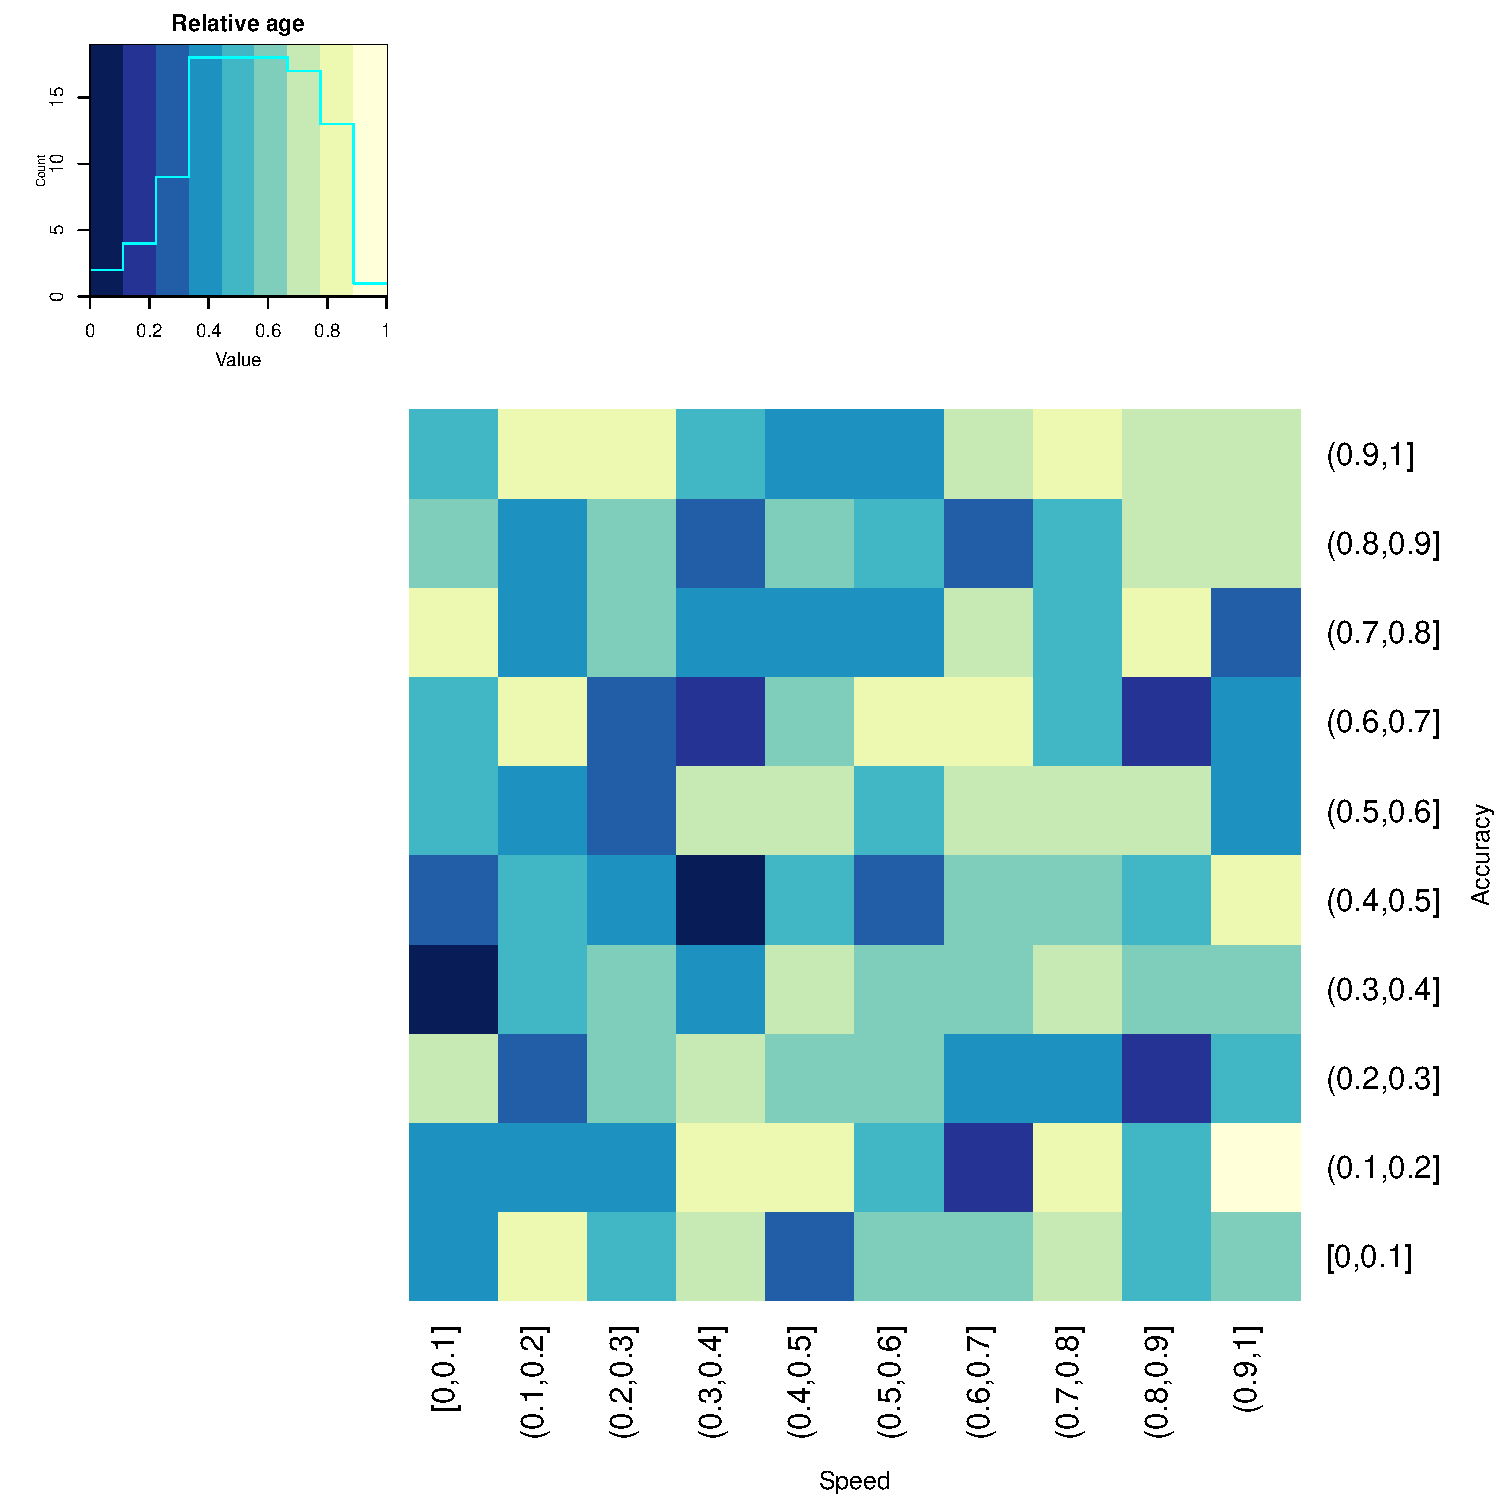
\includegraphics[width=0.45\textwidth]{relAge-SpeedVsAccuracy-heatmap.pdf}\\
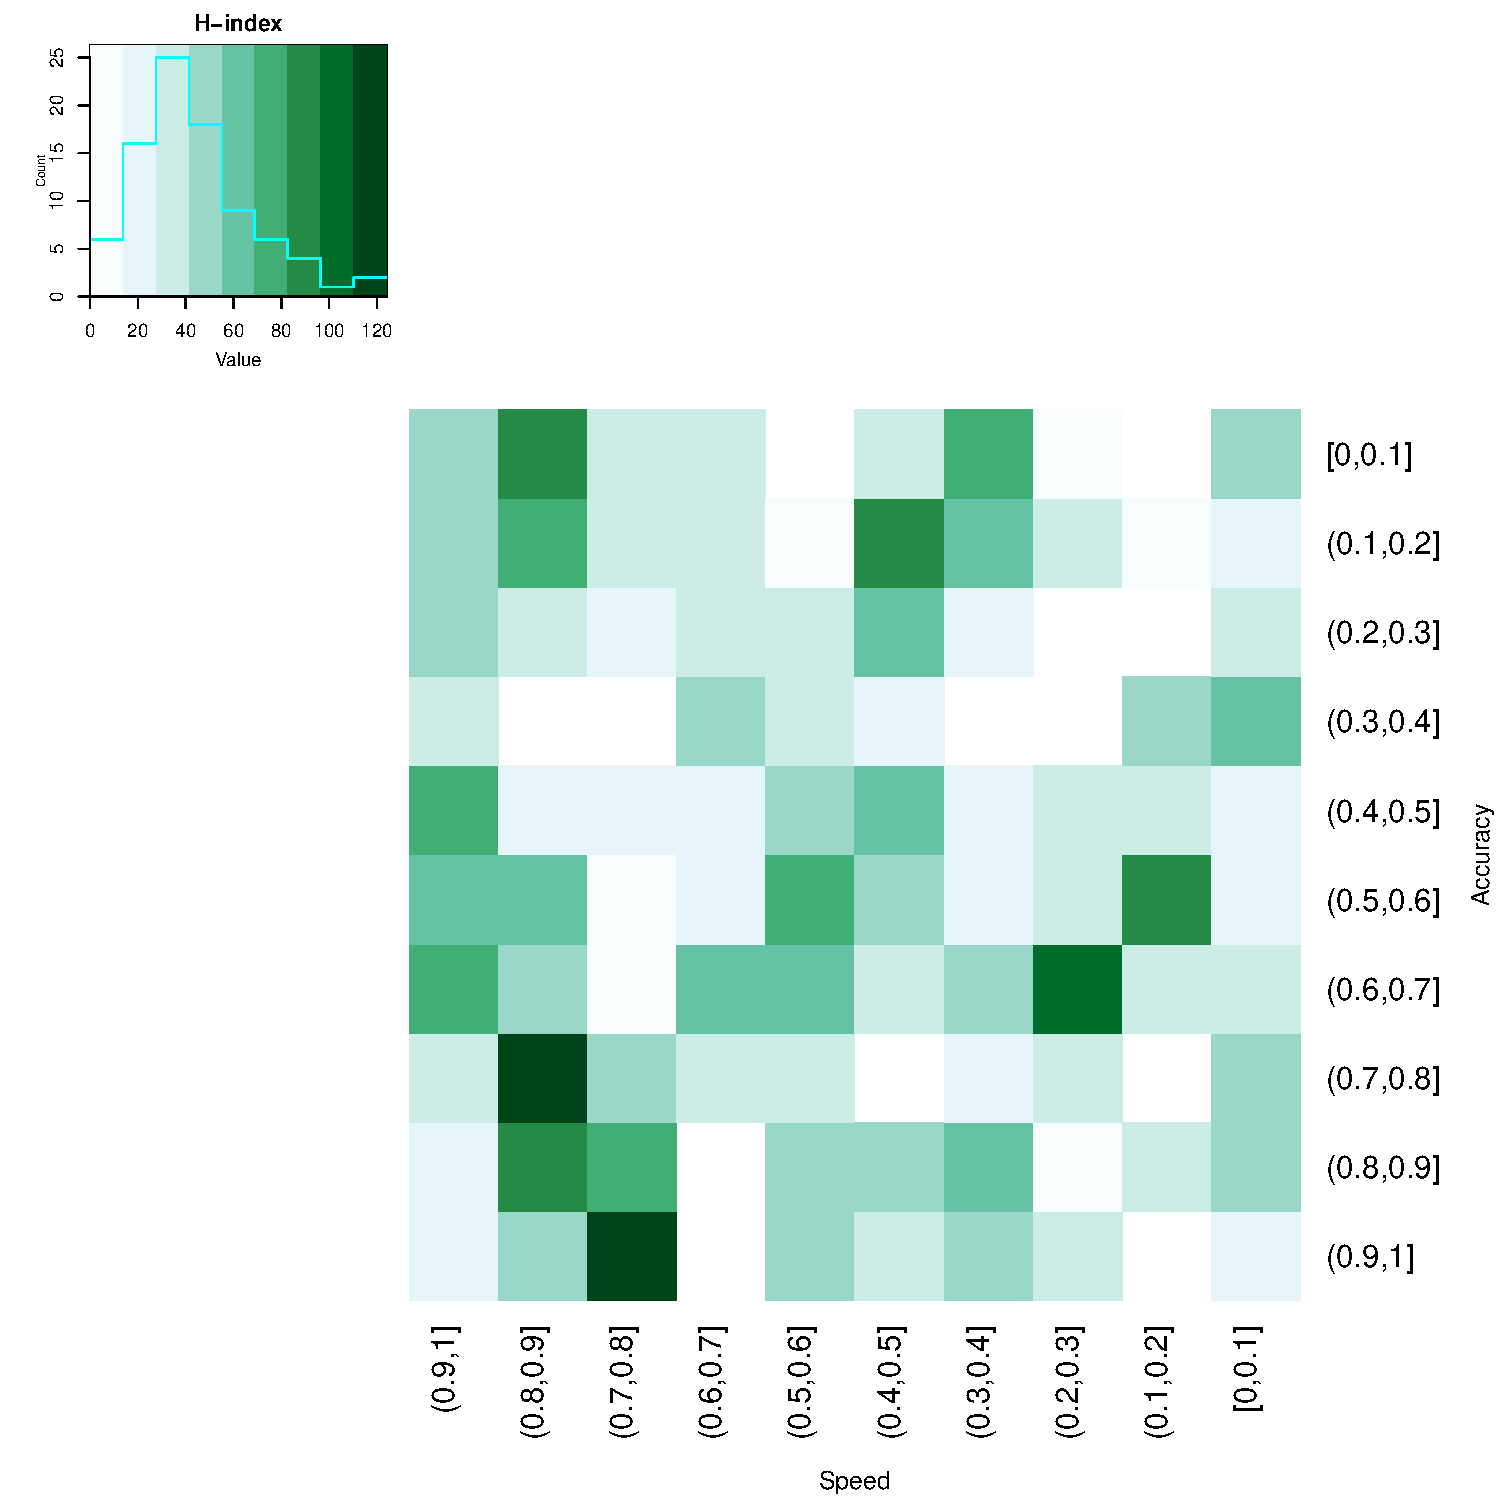
\includegraphics[width=0.45\textwidth]{hindex-SpeedVsAccuracy-heatmap.pdf}
\caption{...}
\label{fig:S4}
\end{figure}


\begin{figure}[H]
\centering
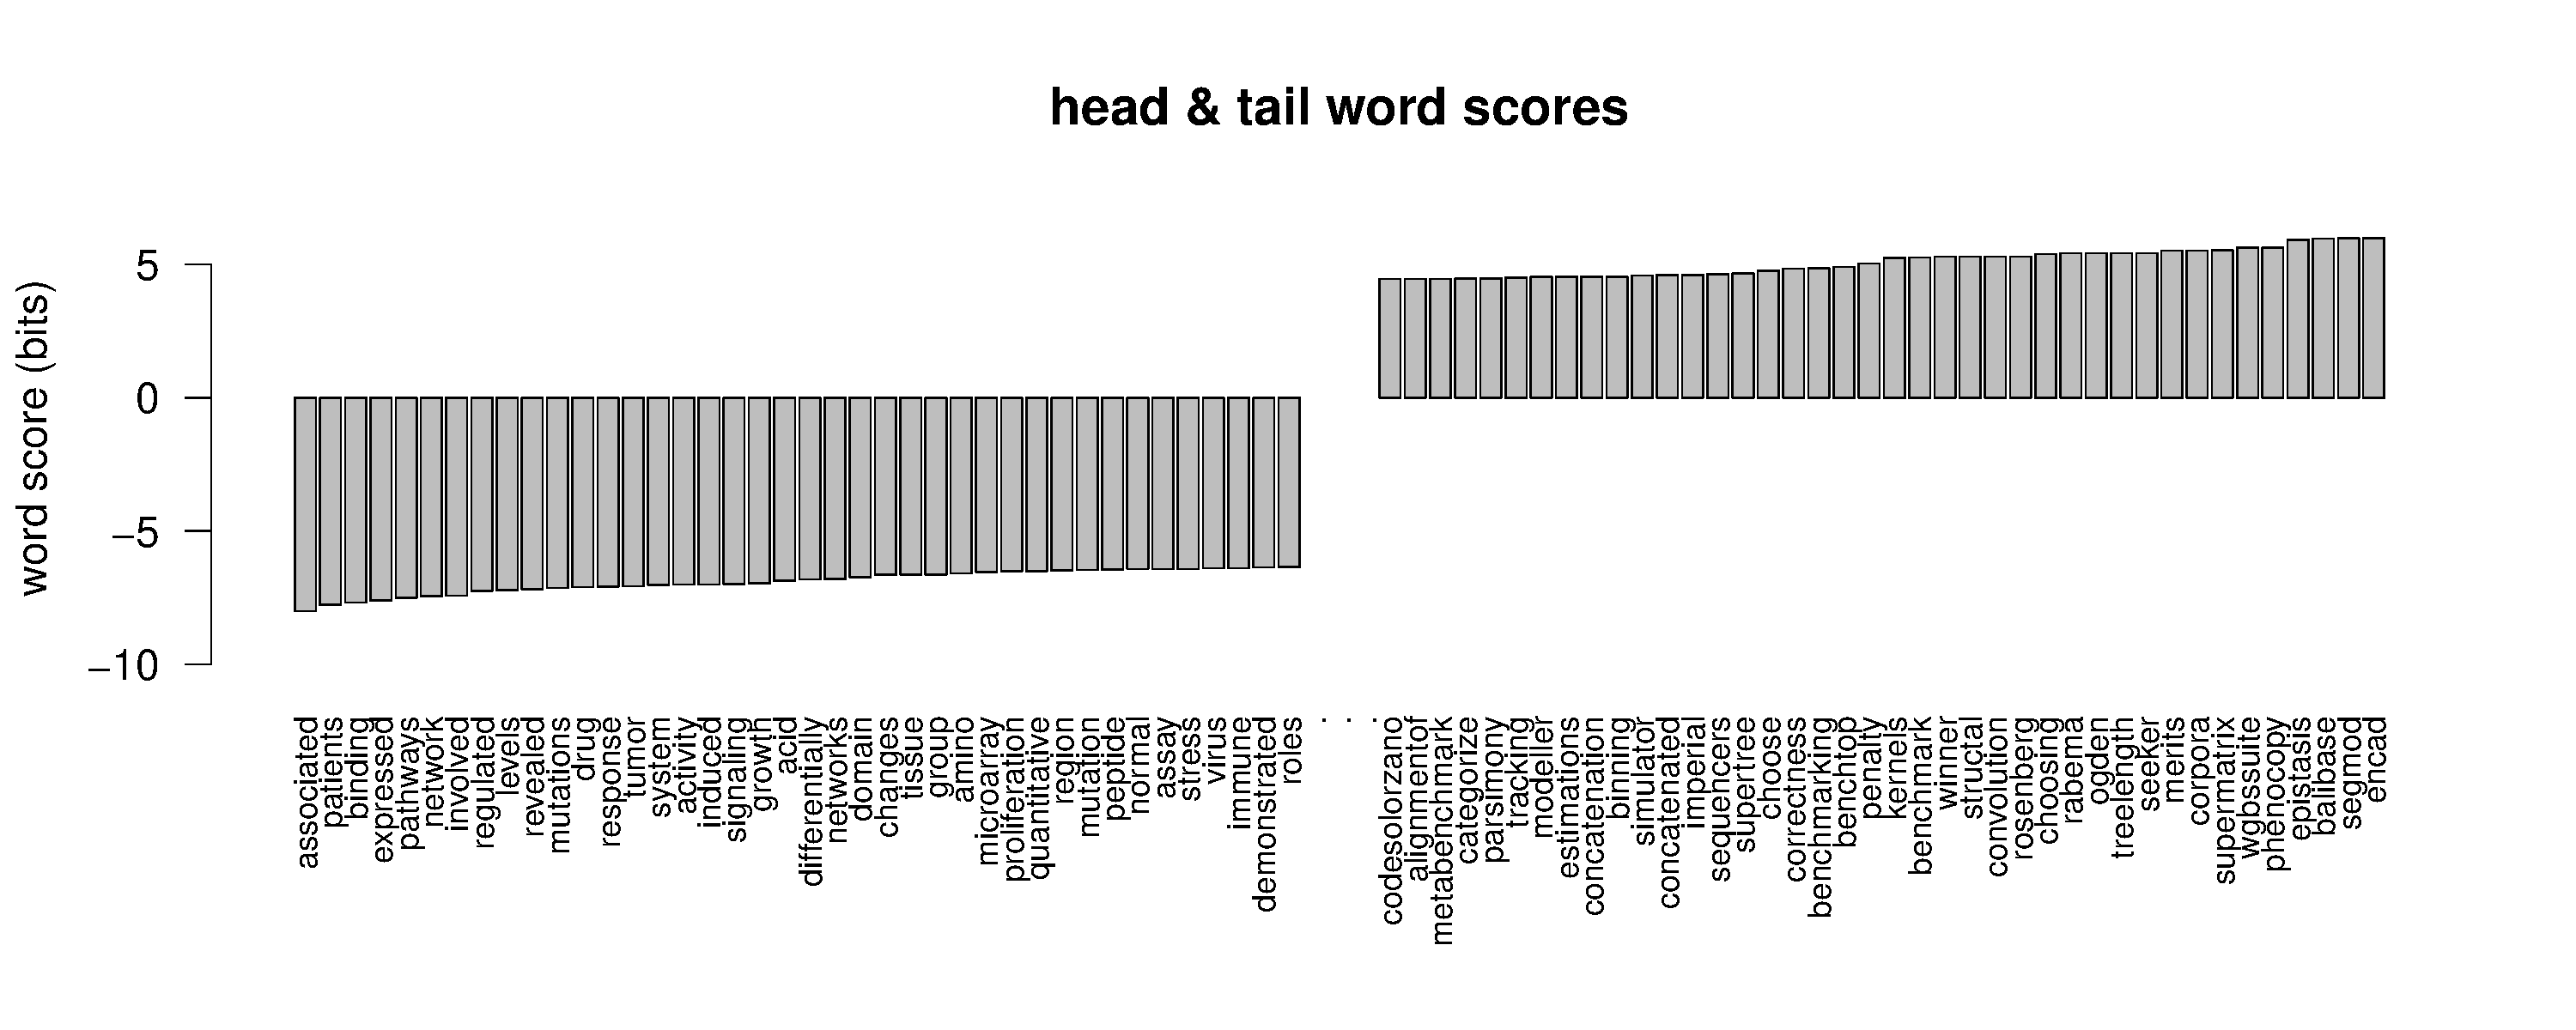
\includegraphics[width=0.85\textwidth]{wordScores.pdf}
\caption{...}
\label{fig:S5}
\end{figure}


%----------------------------------------------------------------------------------------
%	REFERENCE LIST
%----------------------------------------------------------------------------------------
\bibliographystyle{unsrt}
\bibliography{paulall}

\end{document}








